\subsection{XOR en OR}
De verschillen tussen het leren van de XOR en OR operaties worden hier onderzocht. Het enige verschil tussen de twee operaties is dat XOR gemiddeld 0.5 kans heeft dat het antwoord 1 of 0 is. OR heeft gemiddeld 0.75 kans dat het antwoord een 1 is en 0.25 kans dat het 0 is.

\begin{table}[ht]
    \centering
      $\begin{array}{l || c | c | c | c}
                                    & \text{Aantal verborgen knopen} & \text{XOR} & \text{OR} \\ \hline
        \text{Aantal correct}       & \multirow{2}{*}{4}  & 26 & 47 \\ \cline{1-1} \cline{3-4}
        \text{Percentage \% correct} &                    & 52 & 94 \\ \cline{1-1} \cline{3-4} \hline \hline
        \text{Aantal correct}       & \multirow{2}{*}{8} & 31 & 50 \\ \cline{1-1} \cline{3-4}
        \text{Percentage \% correct} &                    & 62 & 100 \\ \cline{1-1} \cline{3-4} \hline
      \end{array}$
    \caption{Aantal correcte antwoorden over 50 executies met operaties XOR en OR met verschillende aantallen verborgen knopen}
    \label{tab:xoror}
\end{table}

\begin{figure}[ht!]
    \centering
    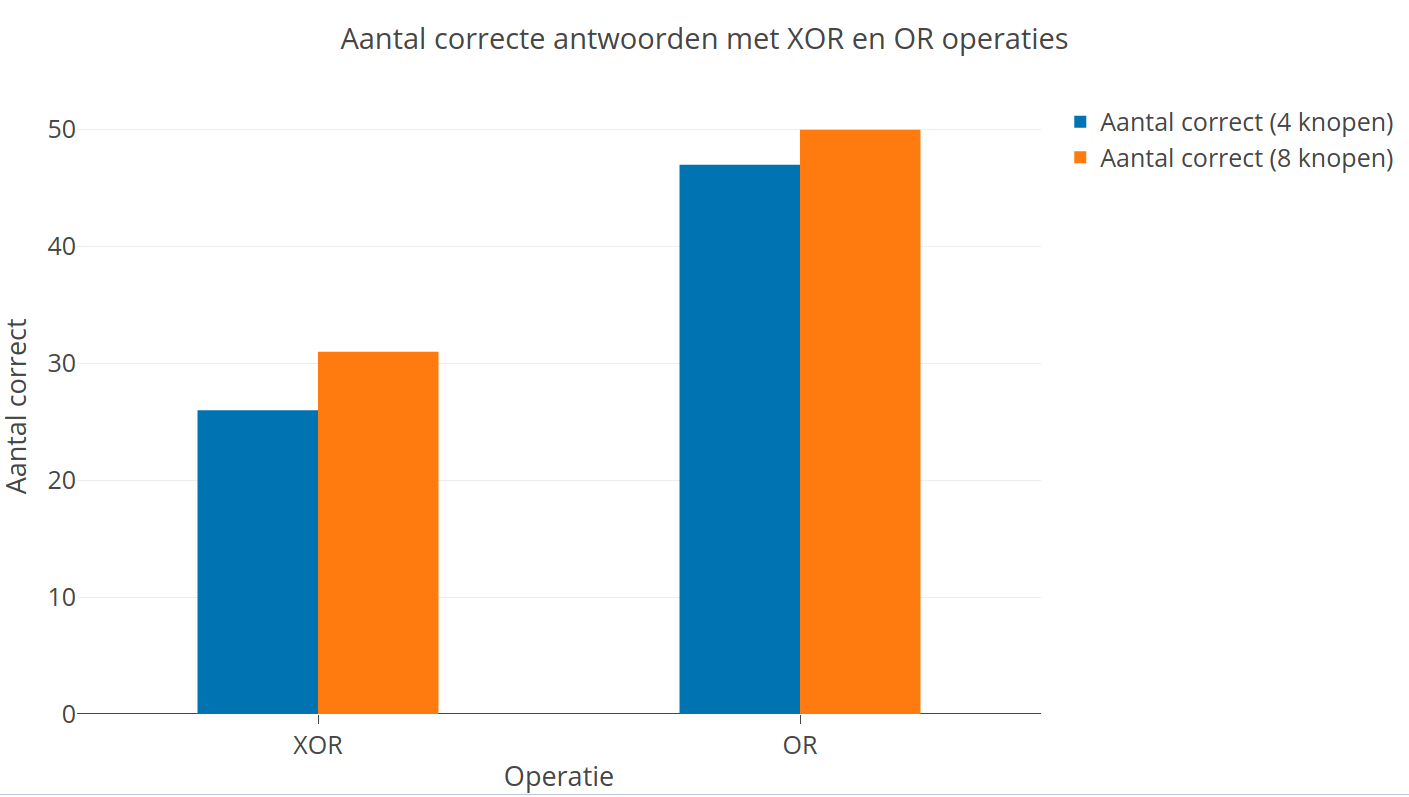
\includegraphics[scale=0.3]{graphs/xoror.png}
    \caption{Aantal correcte antwoorden over 50 executies met operaties XOR en OR met verschillende aantallen verborgen knopen}
    \label{fig:xoror}
\end{figure}

Tabel \ref{tab:xoror} en Figuur \ref{fig:xoror} laat zien hoe goed het netwerk de operaties XOR en OR leert. We zien dat het netwerk de OR operatie beter leert dan de XOR operatie op beide verschillende hoeveelheden knopen. Dit kan komen doordat de kans dat de XOR operatie een 1 of 0 als antwoord heeft, $0.5$ is voor beiden, dus er is meer kans op variatie in de antwoorden die het netwerk moet geven. Voor de OR operatie is dit $0.75$ voor een 1 en $0.25$ voor een 0. Dit zorgt ervoor dat voor de OR operatie het netwerk meer geneigd is om een 1 als antwoord te geven en dus 75\% van de gevallen altijd correct is. Dus de OR operatie zal vaker correct worden beantwoord door het netwerk dan de XOR operatie.
